\documentclass[12pt,reqno]{amsart}
\usepackage{./header, amssymb}

\hdr{Mathematical Statistics}{Chapter 13: Learning}

\begin{document}

\bigskip

\prob Consider a \textit{Naive Bayes model} as described in the programming assignment for chapter 12. The underlying graph is of the form

\bigskip
\begin{center}
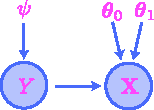
\includegraphics[scale=1.5]{nb}
\end{center}
\bigskip

where $\mathbf{X} \in \mathbb{R}^n$. The parameters are given by a number $\psi\in [0,1]$ which parametrizes the distribution of $Y\sim \mathcal{B}er(\psi)$, as well as two vectors $\boldsymbol{\theta}_0, \boldsymbol{\theta}_1 \in [0,1]^n$. The link function at $\mathbf{X}$ is given by
	\[
	p(\mathbf{x} \mid y ; \  \boldsymbol{\theta}_0, \boldsymbol{\theta}_1 ) = \prod_{j=1}^n \phi_j^{x_j}(1-\phi_j)^{1-x_j}
	\]
where
	\[
	\boldsymbol{\phi} = (1-y) \boldsymbol{\theta}_0 + y \boldsymbol{\theta}_1
	\]
and	$\boldsymbol{\phi}^\intercal = (\phi_1,\ldots,\phi_n)$.

\bigskip
\begin{enumerate}
\item Assuming that Naive Bayes models are trained as \textbf{generative} models, write down a formula for the model likelihood function $\mathcal{L}_\text{model}(\psi,\boldsymbol{\theta}_0,\boldsymbol{\theta}_1)$. For simplicity, your formula should contain the $\phi_j$'s rather than the parameters $\boldsymbol{\theta}_0$ and $\boldsymbol{\theta}_0$ themselves.

\bigskip
\textcolor{red}{We have
	\begin{align*}
	\mathcal{L}_\text{model}(\psi,\boldsymbol{\theta}_0,\boldsymbol{\theta}_1; \ \mathbf{x},y) &= p(\mathbf{x},y; \ \psi, \boldsymbol{\theta}_0, \boldsymbol{\theta}_1) \\
	&= p(y; \psi) p(\mathbf{x}\mid y; \ \boldsymbol{\theta}_0, \boldsymbol{\theta}_1) \\ 
	&= \psi^y(1-\psi)^{1-y} \prod_{j=1}^n \phi_j^{x_j}(1-\phi_j)^{1-x_j}.
	\end{align*}}
\bigskip

\item Using your answer from part (a), write down a formula for the model surprisal function $\mathcal{I}_\text{model}(\psi,\boldsymbol{\theta}_0,\boldsymbol{\theta}_1)$. For simplicity, your formula should contain the $\phi_j$'s rather than the parameters $\boldsymbol{\theta}_0$ and $\boldsymbol{\theta}_0$ themselves.

\bigskip
\textcolor{red}{We have
	\begin{align*}
	\mathcal{I}_\text{model}(\psi,\boldsymbol{\theta}_0,\boldsymbol{\theta}_1; \ \mathbf{x},y) &= - \log{\mathcal{L}_\text{model}(\psi,\boldsymbol{\theta}_0,\boldsymbol{\theta}_1; \ \mathbf{x},y)} \\
	&= - y \log{\psi} - (1-y) \log{(1-\psi)} - \sum_{j=1}^n\left[x_j \log{\phi_j} + (1-x_j) \log{(1-\phi_j)} \right].
	\end{align*}}
\bigskip


\item Using your answer from part (b), write down an explicit formula for the cross entropy stochastic objective function $J(\psi,\boldsymbol{\theta}_0,\boldsymbol{\theta}_1)$ for a dataset of size $m$.

\bigskip
\textcolor{red}{Letting
	\[
	(\mathbf{x}_1,y_1),(\mathbf{x}_2,y_2),\ldots,(\mathbf{x}_m,y_m) \in \{0,1\}^m \times \{0,1\}
	\]
be the dataset, by definition we have
	\begin{align*}
	J(\psi, \boldsymbol{\theta}_0,\boldsymbol{\theta}_1) &= \frac{1}{m} \sum_{i=1}^m \mathcal{I}_\text{model}(\psi,\boldsymbol{\theta}_0,\boldsymbol{\theta}_1; \ \mathbf{x}_i, y_i) \\
	&= \frac{1}{m} \sum_{i=1}^m \left\{ - y_i \log{\psi} - (1-y_i) \log{(1-\psi)} - \sum_{j=1}^n\left[x_{ij} \log{\phi_j} + (1-x_{ij}) \log{(1-\phi_j)} \right]\right\}.
	\end{align*}}
\bigskip
\end{enumerate}








\bigskip
\prob Consider the observed dataset
	\[
	(0, 0), (1, 1), (2,3) \in \mathbb{R}^2.
	\]
Using this dataset, compute the exact MLEs for the parameters $\beta_0$ and $\beta_1$ of a simple linear regression model (with known variance).

\bigskip
\textcolor{red}{We have $\bar{x} = 1$ and $\bar{y} = 4/3$, so
	\[
	(\beta_1)^\star_\text{MLE} = \frac{(0-1)(0-4/3) + (1-1)(1-4/3) + (2-1)(3-4/3)}{(0-1)^2 + (1-1)^2 + (2-1)^2} = \frac{3}{2}
	\]
and
	\[
	(\beta_0)^\star_\text{MLE} = \frac{4}{3} - \frac{3}{2} \cdot 1 = - \frac{1}{6}.
	\]}
\bigskip







\prob For the neural network trained in Section 13.5, compute the following:

\bigskip
\begin{enumerate}
\item The number of gradient steps per epoch.

\bigskip
\textcolor{red}{The dataset has size $m=3{,}072$ and the mini-batch size is $k=128$. Thus, the algorithm takes $3{,}072/128 = 24$ gradient steps per epoch.}
\bigskip

\item The \textit{exact} number of gradient steps over all epochs.

\bigskip
\textcolor{red}{The algorithm takes a total of $80 \times 24 = 1{,}920$ gradient steps.}
\bigskip

\item The number of trainable parameters in the network.

\bigskip
\textcolor{red}{The network has three hidden layers of widths $8$, $8$, and $4$, and an input layer of width $2$. This means we have \textit{four} parameter groups:
	\[
	(\mathbf{W}_1,\mathbf{b}_1),(\mathbf{W}_2,\mathbf{b}_2),(\mathbf{W}_3,\mathbf{b}_3),(\mathbf{w}_4,b_4),
	\]
with
	\[
	\mathbf{W}_1 \in \mathbb{R}^{2\times 8}, \ \mathbf{b}_1 \in \mathbb{R}^8, \ \mathbf{W}_2 \in \mathbb{R}^{8\times 8}, \ \mathbf{b}_2 \in \mathbb{R}^8, \ \mathbf{W}_3 \in \mathbb{R}^{8\times 4}, \ \mathbf{b}_3 \in \mathbb{R}^4, \ \mathbf{w}_4 \in \mathbb{R}^{4}, \ b_4 \in \mathbb{R} .
	\]
So, there are
	\[
	(2\cdot 8) + 8 + (8 \cdot 8) + 8 + (8 \cdot 4) + 4 + 4 + 1 = 137
	\]
trainable parameters.}
\end{enumerate}


\end{document}